\documentclass{article}
\usepackage{hyperref}
\usepackage{float}
\usepackage{tikz}
\usetikzlibrary{arrows.meta, positioning, calc, decorations.pathmorphing, shapes.geometric}
\begin{document}
\section{Implementation Details}

\begin{figure}[H]
    \centering
    
    
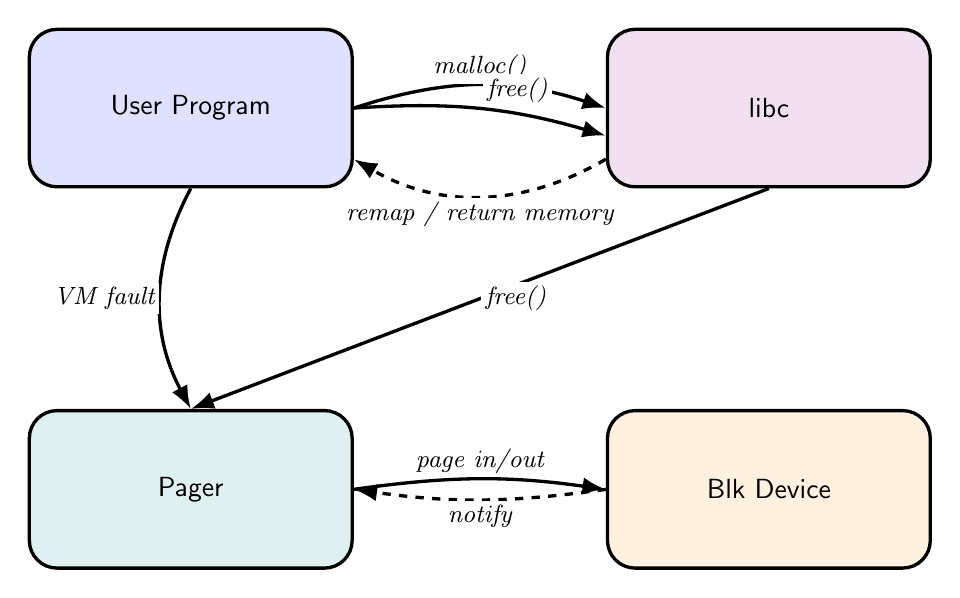
\begin{tikzpicture}[
font=\sffamily,
>=Latex,
node distance=2.8cm and 3.2cm,
box/.style={
draw,
rounded corners=10pt,
very thick,
minimum width=4.1cm,
minimum height=2.0cm,
align=center,
fill=#1!12
},
flow/.style={->, very thick},
backflow/.style={->, very thick, dashed},
lab/.style={midway, fill=white, inner sep=1.5pt, font=\small\itshape}
]

% Nodes
\node[box=blue] (user) {User Program};
\node[box=violet, right=of user] (mm) {libc};
\node[box=teal, below=of user] (page) {Pager};
\node[box=orange, right=of page] (blk) {Blk Device};

% User <-> Memory manager
\draw[flow, bend left=18]
(user.east) to node[lab, above] {malloc()} (mm.west);

\draw[flow, bend left=10]
(user.east) to node[lab, above right] {free()} ($(mm.west)+(0,-0.35)$);

\draw[backflow, bend left=30]
($(mm.west)+(0,-0.65)$) to node[lab, below] {remap / return memory} ($(user.east)+(0,-0.65)$);

% User -> Page fault
\draw[flow, bend right=28]
(user.south) to node[lab, left] {VM fault} (page.north);

% Memory manager -> Page
\draw[flow]
(mm.south) -- node[lab, right] {free()} (page.north);

% Page <-> Block device
\draw[flow, bend left=8]
(page.east) to node[lab, above] {page in/out} (blk.west);

\draw[backflow, bend left=8]
(blk.west) to node[lab, below] {notify} (page.east);

\end{tikzpicture}

\caption{System Diagram for Pager and Memory Manager. Free is not yet implemented.}
\end{figure}
\subsection{Design Problems}
LionsOS is a static operating system. What this means is that all applications and memory regions etc. are loaded before runtime and these applications run for the lifetime of the system. This forms a problem regarding the implementation of the pager and memory manager on LionsOS as the memory manager is supposed to grant extra memory to a protection domain on request. However, where should this memory come from? It is important to note that the microkit currently does not support the retyping of memory in userland. This means that it is impossible without extensively changing microkit to even change the page tables during runtime. 

We can instead premake page tables during compilation for a large area and map and unmap frames and do demand paging to make it seem that there is more memory than there actually is. The frames come from an \textit{unbacked} memory region which is mapped into the pager's vspace and the pager through blk operations can implement demand paging. On compilation, the frame caps can be given to the pager for it to map to the clients' vspaces. \textit{Note: this implementation is only a proof of concept design to run benchmarks to compare paging performance against Linux. A proper design would have the pager deal with untyped memory.}
\subsection{Limitations of the Design}
\begin{itemize}
    \item There is a static upper limit of the number of protection domains that are supported by the pager, defined as \texttt{MAX\_PDS}.
    \item Protection domains that are to be supported by the pager must be specified as `children' of the pager in the system description file.
    \item The `children' of the pager must have an ID less than \texttt{MAX\_PDS}.
    \item The memory manager only allocates 4k size blocks.
    \item The Pager must be named `pager' in the system description file.
    \item The number of available frames is fixed upon loading the system.
    \item The `heap' allocated to by the memory manager always starts at 0x8000000000. (LionsOS libc reflects this).
    \item The `heap' must be specified in the system description file as an unbacked memory region. 
    \item Protection domains are singlethreaded.
    \item `Child' protection domains of the pager do not have other faults except page faults.
    \item There is a static limit to the address space size - demand paging does not mean an infinite address space size. 
\end{itemize} 
\subsection{Sdfgen}
In order to support such a heap described in section 2.1, we need to implement a memory region which actually remains unmapped from the vspace of the protection domain of the client. In order to do this, we need to have a flag in the memory region object of the system description file to mark a memory region to remain unmapped. This memory region also needs to have its frame caps to be accessible by and mapped into the pager protection domain to do paging operations. In order to support this, I have added a new optional boolean field identified as `backed'. By default memory regions are backed=True, and if they are backed=False, mappings are not done, only the page table structures are created, the memory region mapped to a protection domain named `pager' and the frame caps passed to the protection domain named `pager'. Protection domains can be marked as `backed=False' which means that the stack of the protection domain is also unbacked and reliant on the pager using the same memory region's frames.
\\\\
This is implemented in \href{https://github.com/au-ts/microkit_sdf_gen}{sdfgen} in branch `joshua/unbacked\_pd' as an additional optional field in the constructor of \texttt{MemoryRegion}. It is also possible to bypass the sdfgen entirely by writing up the system description file by hand and including an attribute `backed=false' in the memory region xml object.
\subsection{Microkit}
Microkit reads the SDF to load and run the system described in the SDF. I have modified microkit in order to implement the functionality described in the SDF.
\subsubsection{Special Protection Domains}
There are special protection domains which are named as below: \begin{itemize}
    \item pager
\end{itemize}
These are the required components to make the userland pager functional. The microkit when looping through the protection domains whilst building recognises these protection domains by their name string and implements special behaviour for these protection domains.
\paragraph{pager}
The pager needs to have all of the frames of the `heaps' (and stacks if necessary) mapped into its vspace and needs to have all of the frame caps in order to map the frames to the client protection domains' vspaces. Microkit usually loops through the memory regions, creates frame caps for them and maps the frames using these frame caps into their respective protection domains as specified by the mappings in the sdf. The modification which I have made in microkit intercepts the mapping of frames and checks whether or not the memory region is `backed', if not backed, the frame capability is stored in an array alongside with the id of the protection domain which the `heap' is mapped to. The frame is also mapped into the pager. The array is written as a symbol into the pager's elf so that the pager has access to the frame caps.
\subsubsection{Microkit Interface}
Wrapper functions were implemented for seL4\_ARM\_map/unmap functionality in microkit.h to allow the pager to do mapping operations.
\subsection{LionsOS}
LionsOS is used instead of microkit in order to have easier access to drivers through SDDF. 
\subsubsection{User Application}
The user application should be configured with libc. I have modified the memory management code such that the morecore region starts at 0x8000000000 (just an arbitrarily hardcoded number) and thus can be supported by the pager. Normal malloc can be called and this will be supported by the pager. Free is not implemented for libc and also not supported by the pager. Frees will therefore leak memory.
\subsubsection{Pager}
\paragraph{Data Structures}
There are two things the need to be kept track of: \textit{pagefile slots} \& \textit{frames/pages}.\\\\
The way that I keep track of pagefile slots is through an array. The slot index represents the position of the slot in the file. Essentially I abstract the pagefile as an array. There is a counter which represents the highest slot number which has ever been used so if a new file slot is required, that number can be given and incremented up. There is also a stack which track the freed slots from when a page is freed. If a slot is requested, the stack is checked first then the highest slot number is incremented.
\\\\
Instead of keeping track of page table entries as one normally would in a traditional pager implementation, since seL4 does not provide transparency into page tables, I have chosen to keep track of frame caps and a pseudo page table entry. pseudo page table entries are kept in an array of arrays, which are indexed by pd\_idx and address / 4096. The struct carrying the frame caps are what is used in the page replacement algorithm. They are stored in three lists, a free list, an inactive list and an active list.

\paragraph{Two List Page Replacement}
\begin{figure}[H]
    \centering
    \resizebox{1.3\textwidth}{!}{
        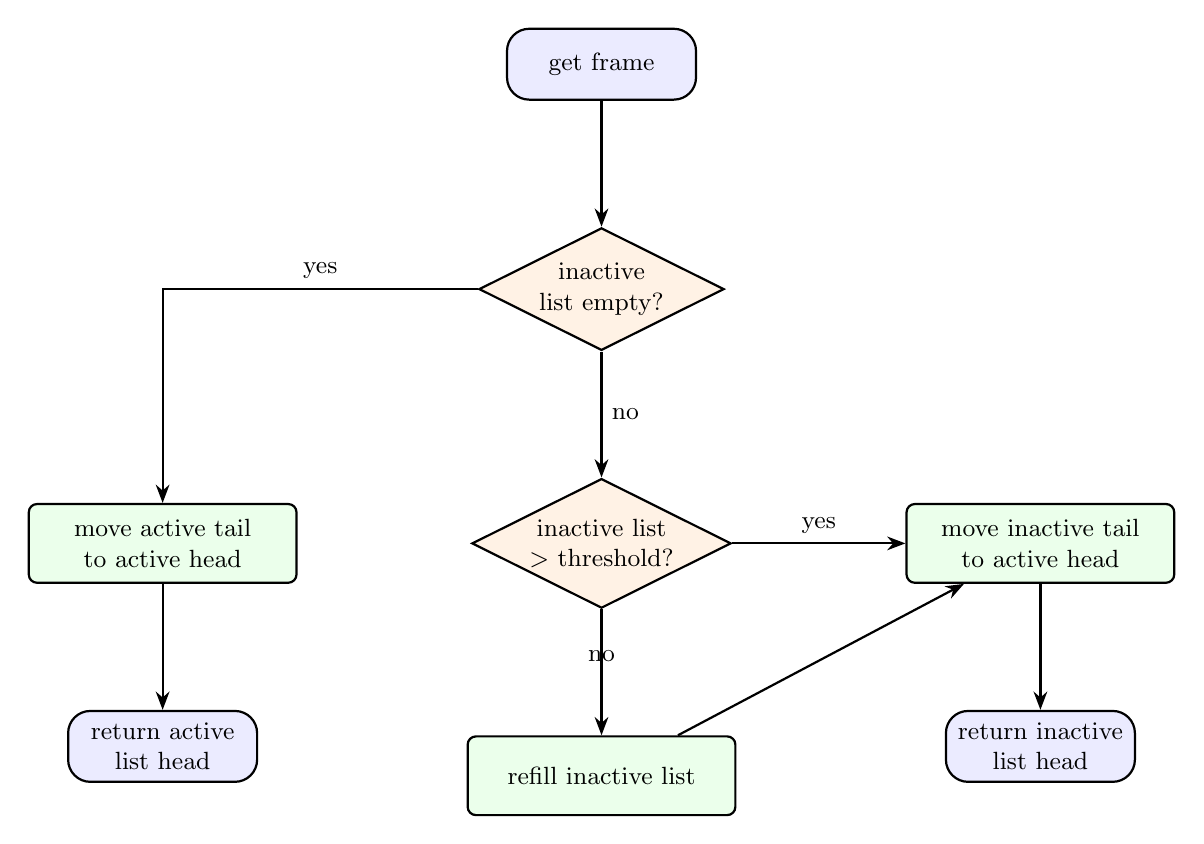
\begin{tikzpicture}[
node distance=16mm and 22mm,
font=\small,
>=Stealth,
startstop/.style={
rectangle, rounded corners=8pt,
draw, thick, align=center,
minimum width=24mm, minimum height=9mm,
fill=blue!8
},
process/.style={
rectangle,
draw, thick, rounded corners=3pt,
align=center,
minimum width=34mm, minimum height=10mm,
fill=green!8
},
decision/.style={
diamond,
draw, thick,
aspect=2,
align=center,
inner sep=1pt,
fill=orange!10
},
arrow/.style={->, thick}
]

\node[startstop] (start) {get frame};

\node[decision, below=of start] (inactiveEmpty)
{inactive\\list empty?};

\node[decision, below=of inactiveEmpty] (inactiveBig)
{inactive list\\$>$ threshold?};

\node[process, right=of inactiveBig] (moveInactive)
{move inactive tail\\to active head};

\node[startstop, below=of moveInactive] (returnInactive)
{return inactive\\list head};

\node[process, below=of inactiveBig] (refill)
{refill inactive list};

\node[process, left=of inactiveBig] (moveActive)
{move active tail\\to active head};

\node[startstop, below=of moveActive] (returnActive)
{return active\\list head};

\draw[arrow] (start) -- (inactiveEmpty);

\draw[arrow] (inactiveEmpty) -- node[right] {no} (inactiveBig);
\draw[arrow] (inactiveEmpty.west) -| node[pos=0.25, above] {yes} (moveActive.north);

\draw[arrow] (inactiveBig) -- node[above] {yes} (moveInactive);
\draw[arrow] (inactiveBig) -- node[above] {no} (refill);

\draw[arrow] (refill) -- (moveInactive);

\draw[arrow] (moveInactive) -- (returnInactive);

\draw[arrow] (moveActive) -- (returnActive);

\end{tikzpicture}


    }
    
\end{figure}
The entry point for the two list page replacement algorithm is the \texttt{get\_frame()} function which returns the next frame which could be used. This frame may or may not be already mapped to a page, but the pager takes care of that. The refill inactive function basically loops around the active list and if the current node's reference bit is set, sets this to false and unmaps and pushes to front of active list. If the current node is dereferenced then it is pushed to the front of the inactive list.
\paragraph{Paging Flow}
\begin{figure}[H]
    \centering
    \resizebox{1.3\textwidth}{!}{
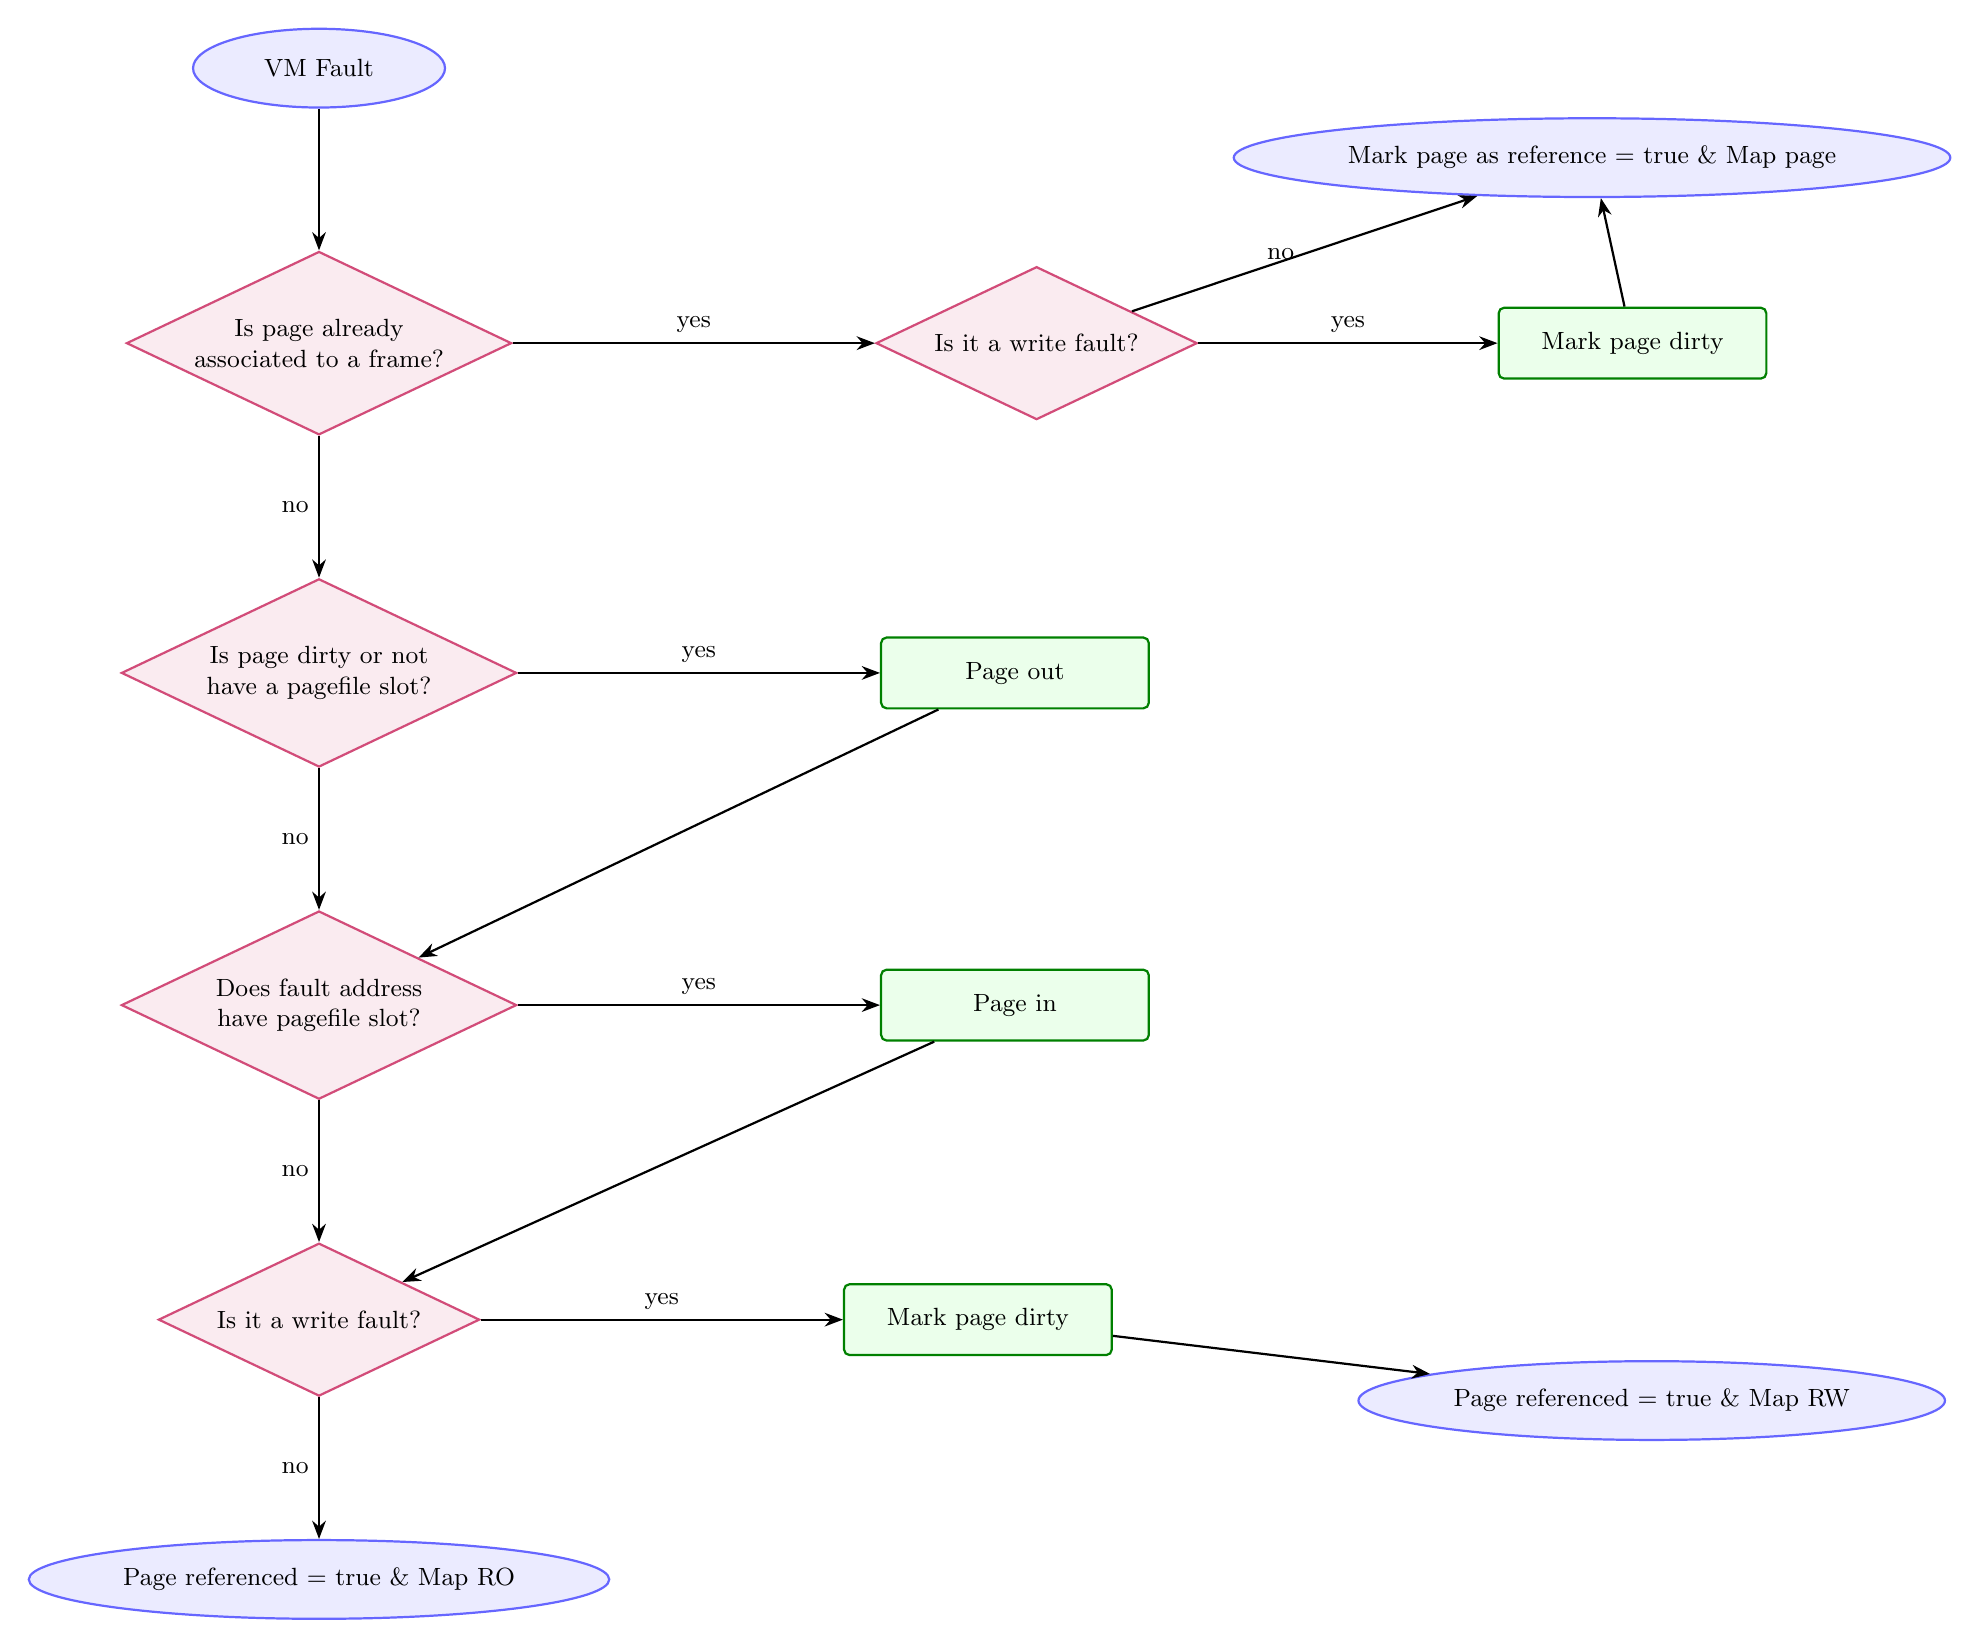
\begin{tikzpicture}[
node distance=1.8cm and 3.2cm,
>=Stealth,
every node/.style={font=\small},
startstop/.style={
ellipse,
draw=blue!60,
fill=blue!8,
thick,
minimum width=3.2cm,
minimum height=1cm
},
decision/.style={
diamond,
draw=purple!70,
fill=purple!8,
thick,
aspect=2.1,
inner sep=1pt,
text width=3.4cm,
align=center
},
process/.style={
rectangle,
rounded corners=2pt,
draw=green!50!black,
fill=green!8,
thick,
minimum width=3.4cm,
minimum height=0.9cm,
text centered
},
line/.style={draw, thick, ->}
]

% Nodes
\node[startstop] (fault) {VM Fault};

\node[decision, below=of fault] (assoc)
{Is page already associated to a frame?};

\node[decision, right=4.6cm of assoc] (writefault1)
{Is it a write fault?};

\node[startstop, above right=1.5cm and 2.8cm of writefault1] (mapframe)
{Mark page as reference = true \& Map page};

\node[process, right=3.8cm of writefault1] (dirty1)
{Mark page dirty};

\node[decision, below=of assoc] (pagedout)
{Is page dirty or not have a pagefile slot?};

\node[process, right=4.6cm of pagedout] (pageout)
{Page out};

\node[decision, below=of pagedout] (slot)
{Does fault address have pagefile slot?};

\node[process, right=4.6cm of slot] (pagein)
{Page in};

\node[decision, below=of slot] (writefault2)
{Is it a write fault?};

\node[process, right=4.6cm of writefault2] (dirty2)
{Mark page dirty};

\node[startstop, below right=0.2cm and 4.2cm of dirty2] (maprw)
{Page referenced = true \& Map RW};

\node[startstop, below=1.8cm of writefault2] (mapro)
{Page referenced = true \& Map RO};

% Connections
\draw[line] (fault) -- (assoc);

% already associated branch
\draw[line] (assoc) -- node[above] {yes} (writefault1);

\draw[line] (writefault1) -- node[above] {yes} (dirty1);
\draw[line] (dirty1) -- (mapframe);

\draw[line] (writefault1) -- node[left] {no} (mapframe);

% not associated branch
\draw[line] (assoc) -- node[left] {no} (pagedout);

\draw[line] (pagedout) -- node[above] {yes} (pageout);
\draw[line] (pageout) -- (slot);

\draw[line] (pagedout) -- node[left] {no} (slot);

\draw[line] (slot) -- node[above] {yes} (pagein);
\draw[line] (pagein) -- (writefault2);

\draw[line] (slot) -- node[left] {no} (writefault2);

\draw[line] (writefault2) -- node[above] {yes} (dirty2);
\draw[line] (dirty2) -- (maprw);

\draw[line] (writefault2) -- node[left] {no} (mapro);

\end{tikzpicture}}
\end{figure}
Paging follows the flow shown above, except that paging in and out operations are done asynchronously through the blk driver. We facilitate this by having a \texttt{page\_continuations} array which allows the pager to index into using the child id and store the paging data which contains the frame, child id, fault address and a enum which tells the pager when notified that the blk operation is finished whether it was a page in or out. There is also a similar array of integers named \texttt{current\_faults} also indexed by child id that stores the fault address to make sure that the current fault is not serviced multiple times. Since we assume that PD's are singlethreaded, there should only be one VM fault happening at any time for a single PD. 

\section{More Detailed System Diagram}


\begin{figure}[ht]
\centering
\resizebox{400pt}{!}{
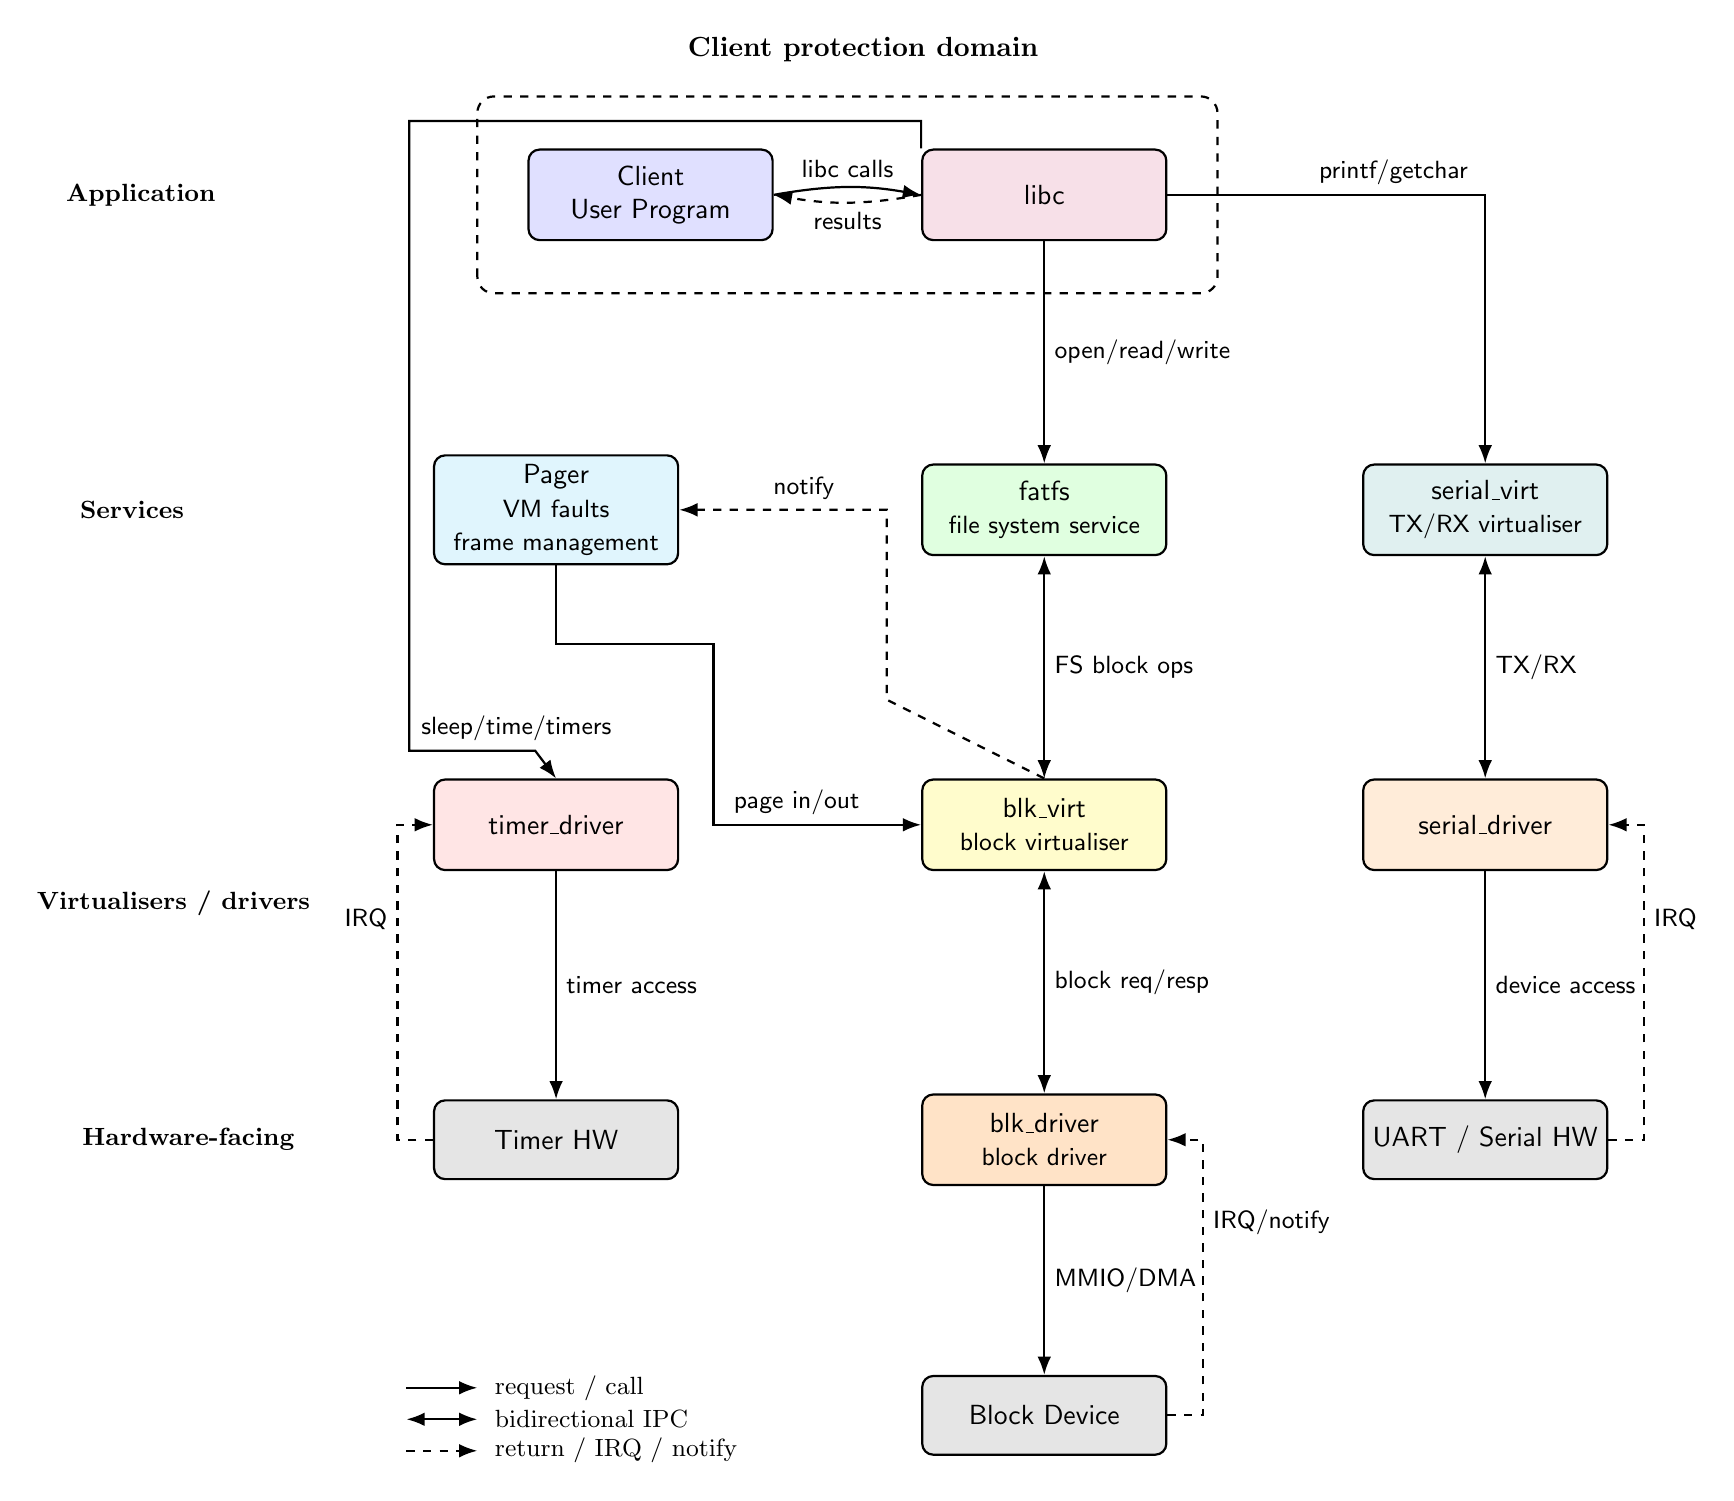
\begin{tikzpicture}[
    font=\sffamily,
    box/.style={
        draw,
        thick,
        rounded corners=4pt,
        minimum width=3.1cm,
        minimum height=1.15cm,
        align=center
    },
    libcbox/.style={
        draw,
        thick,
        rounded corners=4pt,
        minimum width=3.1cm,
        minimum height=1.15cm,
        align=center
    },
    hwbox/.style={
        draw,
        thick,
        rounded corners=4pt,
        minimum width=3.1cm,
        minimum height=1cm,
        align=center,
        fill=gray!20
    },
    arrow/.style={
        ->,
        thick,
        >=Latex
    },
    both/.style={
        <->,
        thick,
        >=Latex
    },
    dashedarrow/.style={
        ->,
        thick,
        dashed,
        >=Latex
    },
    boundary/.style={
        dashed,
        thick,
        rounded corners=6pt
    }
]

% =================================================
% Coordinates
% =================================================

% Main columns:
% x = -5.0 : timer / pager side
% x =  0.5 : client / filesystem / block side
% x =  5.8 : serial side

% =================================================
% Client protection domain
% =================================================

\node[box, fill=blue!12] (client) at (-3.8,5.0)
{Client\\User Program};

\node[libcbox, fill=purple!12] (libc) at (1.2,5.0)
{libc};

\draw[boundary]
    (-6,3.75) rectangle (3.4,6.25);

\node[font=\bfseries] at (-1.1,6.85)
{Client protection domain};

% =================================================
% Service layer
% =================================================

\node[box, fill=cyan!12] (pager) at (-5.0,1.0)
{Pager\\{\small VM faults}\\{\small frame management}};

\node[box, fill=green!12] (fatfs) at (1.2,1.0)
{fatfs\\{\small file system service}};

\node[box, fill=teal!12] (serialvirt) at (6.8,1.0)
{serial\_virt\\{\small TX/RX virtualiser}};

% =================================================
% Driver / virtualisation layer
% =================================================

\node[box, fill=red!10] (timerdrv) at (-5.0,-3.0)
{timer\_driver};

\node[box, fill=yellow!20] (blkvirt) at (1.2,-3.0)
{blk\_virt\\{\small block virtualiser}};

\node[box, fill=orange!15] (serialdrv) at (6.8,-3.0)
{serial\_driver};

% =================================================
% Hardware layer
% =================================================

\node[hwbox] (timerhw) at (-5.0,-7.0)
{Timer HW};

\node[box, fill=orange!22] (blkdrv) at (1.2,-7.0)
{blk\_driver\\{\small block driver}};

\node[hwbox] (uart) at (6.8,-7.0)
{UART / Serial HW};

\node[hwbox] (blkdev) at (1.2,-10.5)
{Block Device};

% =================================================
% App <-> libc
% =================================================

\draw[arrow, bend left=10]
    (client.east) to
    node[above] {\small libc calls}
    (libc.west);

\draw[dashedarrow, bend left=10]
    (libc.west) to
    node[below] {\small results}
    (client.east);

% =================================================
% Memory / pager path
% =================================================

% =================================================
% Filesystem and block path
% =================================================

\draw[arrow]
    (libc.south) --
    node[right] {\small open/read/write}
    (fatfs.north);

\draw[both]
    (fatfs.south) --
    node[right] {\small FS block ops}
    (blkvirt.north);

\draw[arrow]
    (pager.south) -- ++(0,-1) -| ++(2,0) |-
    node[pos=0.7,above] {\small page in/out}
    (blkvirt.west);

\draw[dashedarrow]
    (blkvirt.north) -- ++(-2,1) -| ++(0,1) |- 
    node[pos=0.7,above] {\small notify}
    (pager.east);

\draw[both]
    (blkvirt.south) --
    node[right] {\small block req/resp}
    (blkdrv.north);

\draw[arrow]
    (blkdrv.south) --
    node[right] {\small MMIO/DMA}
    (blkdev.north);

\draw[dashedarrow]
    (blkdev.east) -- ++(0.45,0) |- 
    node[pos=0.35,right] {\small IRQ/notify}
    (blkdrv.east);

% =================================================
% Serial path
% =================================================

\draw[arrow]
    (libc.east) -- ++(0.8,0) -| 
    node[pos=0.32,above] {\small printf/getchar}
    (serialvirt.north);

\draw[both]
    (serialvirt.south) --
    node[right] {\small TX/RX}
    (serialdrv.north);

\draw[arrow]
    (serialdrv.south) --
    node[right] {\small device access}
    (uart.north);

\draw[dashedarrow]
    (uart.east) -- ++(0.45,0) |- 
    node[pos=0.35,right] {\small IRQ}
    (serialdrv.east);

% =================================================
% Timer path routed around outside
% =================================================

\draw[arrow]
    (libc.north west)
    -- ++(0,0.35)
    -- ++(-6.5,0)
    -- ++(0,-8.0)
    -- ++(1.6,0)
    node[pos=0.85,above] {\small sleep/time/timers}
    -- (timerdrv.north);

\draw[arrow]
    (timerdrv.south) --
    node[right] {\small timer access}
    (timerhw.north);

\draw[dashedarrow]
    (timerhw.west) -- ++(-0.45,0) |- 
    node[pos=0.35,left] {\small IRQ}
    (timerdrv.west);

% =================================================
% Layer labels
% =================================================

\node[font=\bfseries\small, anchor=east] at (-9.2,5.0) {Application};
\node[font=\bfseries\small, anchor=east] at (-9.6,1.0) {Services};
\node[font=\bfseries\small, anchor=east] at (-8,-4.0) {Virtualisers / drivers};
\node[font=\bfseries\small, anchor=east] at (-8.2,-7.0) {Hardware-facing};

% =================================================
% Legend
% =================================================

\draw[arrow] (-6.9,-10.15) -- (-6.0,-10.15);
\node[anchor=west, font=\small] at (-5.9,-10.15) {request / call};

\draw[both] (-6.9,-10.55) -- (-6.0,-10.55);
\node[anchor=west, font=\small] at (-5.9,-10.55) {bidirectional IPC};

\draw[dashedarrow] (-6.9,-10.95) -- (-6.0,-10.95);
\node[anchor=west, font=\small] at (-5.9,-10.95) {return / IRQ / notify};

\end{tikzpicture}}
\end{figure}

\end{document}